% Asset ID: FA22ChiSquaredTestsTikZ-002
% Topic ID: FA22ChiSquaredTests
% Unit: FA22 Further A2 2 Applied Mathematics
% Topic code: FA22-CHI2
% Related lesson file: FA22_chi_squared_tests_lesson.md
% Source: CCEA FA22-CHI2 specification + contingency-table evidence
% Purpose: Structure of a contingency table and expected-frequency formula.
\documentclass[tikz,border=8pt]{standalone}
\usepackage{amsmath,xcolor}
\definecolor{Canvas}{HTML}{FAF9F6}\definecolor{Ivory}{HTML}{FFFFF0}\definecolor{Line}{HTML}{E5E5EA}\definecolor{Gold}{HTML}{C5A059}\definecolor{SoftPink}{HTML}{FBEFEF}\definecolor{Text}{HTML}{2C2C2E}
\begin{document}
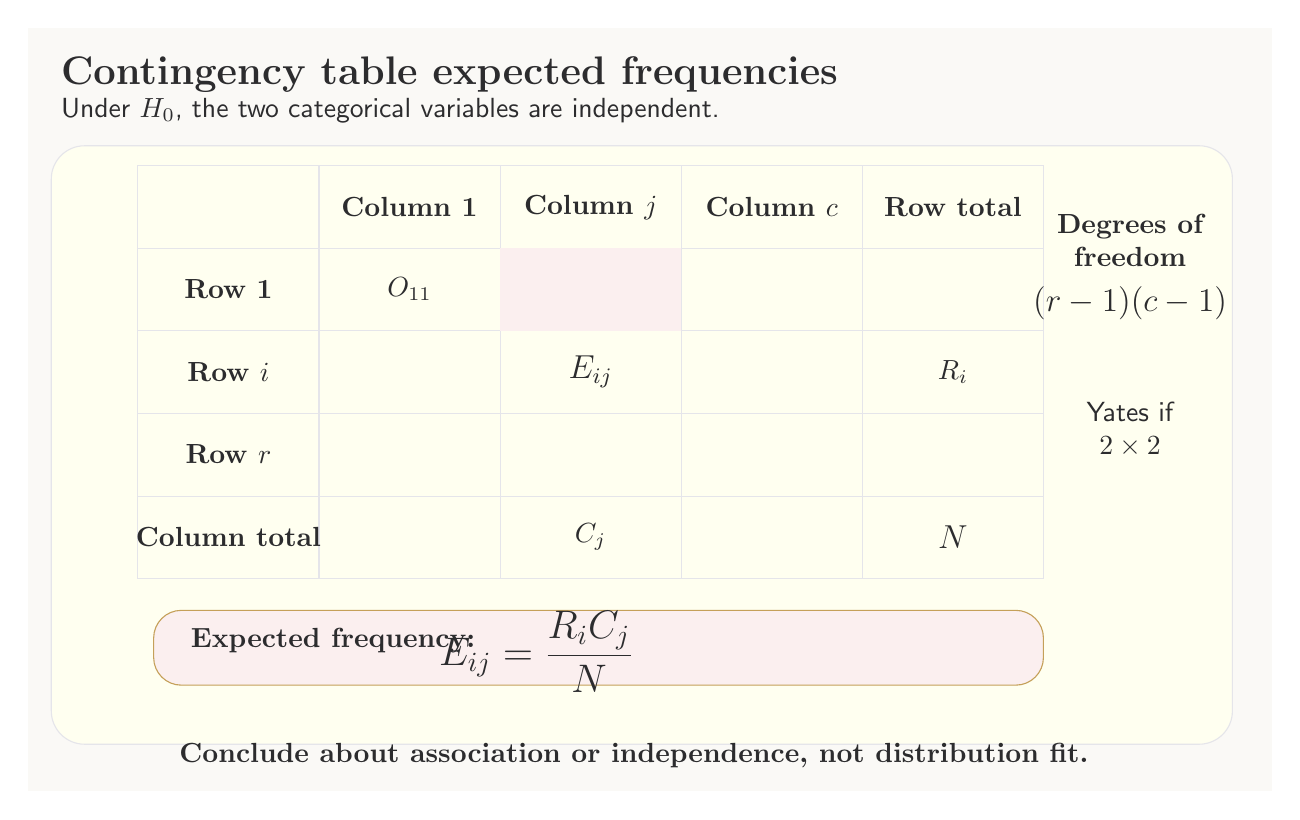
\begin{tikzpicture}[font=\sffamily,every node/.style={text=Text}]
\fill[Canvas] (-1,-1.2) rectangle (14.8,8.5);
\node[anchor=west,font=\bfseries\Large] at (-0.7,7.9){Contingency table expected frequencies};
\node[anchor=west] at (-0.7,7.45){Under \(H_0\), the two categorical variables are independent.};
\filldraw[fill=Ivory,draw=Line,rounded corners=12pt] (-0.7,-0.6) rectangle (14.3,7.0);
\draw[Gold] (0.4,1.5) rectangle (11.9,6.75);
\foreach \x in {0.4,2.7,5.0,7.3,9.6,11.9}{\draw[Line] (\x,1.5)--(\x,6.75);} 
\foreach \y in {1.5,2.55,3.6,4.65,5.7,6.75}{\draw[Line] (0.4,\y)--(11.9,\y);} 
\fill[SoftPink] (5.0,4.65) rectangle (7.3,5.7);
\node at (1.55,6.22){ };\node[font=\bfseries] at (3.85,6.22){Column 1};\node[font=\bfseries] at (6.15,6.22){Column \(j\)};\node[font=\bfseries] at (8.45,6.22){Column \(c\)};\node[font=\bfseries] at (10.75,6.22){Row total};
\node[font=\bfseries] at (1.55,5.18){Row 1};\node[font=\bfseries] at (1.55,4.13){Row \(i\)};\node[font=\bfseries] at (1.55,3.08){Row \(r\)};\node[font=\bfseries] at (1.55,2.03){Column total};
\node at (3.85,5.18){\(O_{11}\)};\node[font=\bfseries\large] at (6.15,4.13){\(E_{ij}\)};\node[font=\bfseries] at (10.75,4.13){\(R_i\)};\node[font=\bfseries] at (6.15,2.03){\(C_j\)};\node[font=\bfseries\large] at (10.75,2.03){\(N\)};
\filldraw[fill=SoftPink,draw=Gold,rounded corners=10pt] (0.6,0.15) rectangle (11.9,1.1);\node[anchor=west,font=\bfseries] at (0.95,0.72){Expected frequency:};\node[anchor=west,font=\Large] at (4.1,0.57){\(E_{ij}=\dfrac{R_iC_j}{N}\)};
\node[align=center,font=\bfseries] at (13.0,5.8){Degrees of\\freedom};\node[align=center,font=\large] at (13.0,5.0){\((r-1)(c-1)\)};\node[align=center] at (13.0,3.4){Yates if\\\(2\times2\)};
\node[font=\bfseries] at (6.7,-0.75){Conclude about association or independence, not distribution fit.};
\end{tikzpicture}
\end{document}
